\documentclass[11pt]{exam}
\usepackage[margin=1in]{geometry}
\usepackage{amsfonts, amsmath, amssymb, amsthm}
\usepackage{mathtools}
\usepackage{enumerate}
\usepackage{listings}
\usepackage{colortbl}
\usepackage{float}
\usepackage{algorithm}
\usepackage{algorithmic}
\usepackage[colorlinks,linkcolor=blue]{hyperref}
\usepackage{graphics}
%%\usepackage{JI_MathCourse_Notations}

% in order to compile this file you need to get 'header.tex' from
% Canvas and change the line below to the appropriate file path
%%% theorems

\theoremstyle{plain}            % following are "theorem" style
\newtheorem{theorem}{Theorem}[section]
\newtheorem{lemma}[theorem]{Lemma}
\newtheorem{corollary}[theorem]{Corollary}
\newtheorem{proposition}[theorem]{Proposition}
\newtheorem{claim}[theorem]{Claim}
\newtheorem{fact}[theorem]{Fact}
\newtheorem{openproblem}[theorem]{Open Problem}

\theoremstyle{definition}       % following are def style
\newtheorem{definition}[theorem]{Definition}
\newtheorem{conjecture}[theorem]{Conjecture}
\newtheorem{example}[theorem]{Example}
\newtheorem{protocol}[theorem]{Protocol}
\newtheorem{exercise}[theorem]{Exercise}

\theoremstyle{remark}           % following are remark style
\newtheorem{remark}[theorem]{Remark}
\newtheorem{note}[theorem]{Note}
%\newtheorem*{solution}{Solution}

%%% special sets
\newcommand{\bit}{\ensuremath{\{0,1\}}}
\newcommand{\bitt}{\ensuremath{\{-1,1\}}}
\newcommand{\ball}{\ensuremath{\mathcal{B}}}
\newcommand{\sph}{\ensuremath{\mathbb{S}}}
\newcommand{\odisc}[2]{\ensuremath{D(#1, #2)}}
\newcommand{\cdisc}[2]{\ensuremath{\bar{D}(#1, #2)}}
\newcommand{\emp}{\varnothing}

% constants
\newcommand{\E}{\ensuremath{\mathrm{e}}}
\newcommand{\I}{\ensuremath{\mathrm{i}}}
\newcommand{\Id}{\ensuremath{\mathrm{I}}}
\newcommand{\paulix}{\ensuremath{\mathrm{X}}}
\newcommand{\pauliy}{\ensuremath{\mathrm{Y}}}
\newcommand{\pauliz}{\ensuremath{\mathrm{Z}}}

% font for general-purpose algorithms
\newcommand{\algo}[1]{\ensuremath{\mathsf{#1}}}
% font for general-purpose computational problems
\newcommand{\problem}[1]{\ensuremath{\mathsf{#1}}}
% font for complexity classes
\newcommand{\class}[1]{\ensuremath{\mathsf{#1}}}

% asymptotics
\DeclareMathOperator{\poly}{poly}
\DeclareMathOperator{\polylog}{polylog}
\DeclareMathOperator{\negl}{negl}
\DeclareMathOperator{\bigO}{O}
\DeclareMathOperator{\litO}{o}
\DeclareMathOperator{\Otil}{\tilde{O}}
\DeclareMathOperator{\Ostar}{O^*}

%%% "LEFT-RIGHT" PAIRS OF SYMBOLS

% inner product
\DeclarePairedDelimiter\inner{\langle}{\rangle}
% absolute value
\DeclarePairedDelimiter\abs{\lvert}{\rvert}
% a set
\DeclarePairedDelimiter\set{\{}{\}}
% parens
\DeclarePairedDelimiter\parens{(}{)}
% tuple, alias for parens
\DeclarePairedDelimiter\tuple{(}{)}
% square brackets
\DeclarePairedDelimiter\bracks{[}{]}
% rounding off
\DeclarePairedDelimiter\round{\lfloor}{\rceil}
% floor function
\DeclarePairedDelimiter\floor{\lfloor}{\rfloor}
% ceiling function
\DeclarePairedDelimiter\ceil{\lceil}{\rceil}
% length of some vector, element
\DeclarePairedDelimiter\length{\lVert}{\rVert}
% "lifting" of a residue class
\DeclarePairedDelimiter\lift{\llbracket}{\rrbracket}
\DeclarePairedDelimiter\len{\lvert}{\rvert}
% bra-kets
\DeclarePairedDelimiter\bra{\langle}{\rvert}
\DeclarePairedDelimiter\ket{\lvert}{\rangle}
\newcommand{\braket}[2]{\ensuremath{\langle #1 \vert #2 \rangle}}
\newcommand{\ketbra}[2]{\ensuremath{\lvert #1 \rangle \langle #2 \rvert}}

%%% spacing

\newcommand{\ws}{\hspace{1pt}}
\newcommand{\wws}{\hspace{2pt}}
\newcommand{\hs}{\hspace{4pt}}
\newcommand{\hhs}{\hspace{8pt}}
\newcommand{\hhhs}{\hspace{12pt}}

%%% LISTS

\newcommand{\oneto}{1, \ldots,}
\newcommand{\onetop}{1 \cdots,}
\newcommand{\zeroto}{0, \ldots,}
\newcommand{\zerotop}{0 \cdots,}
\newcommand{\perm}[1]{\mathbf{(#1)}}
\newcommand{\permv}[1]{(#1)}
\newcommand{\varind}[2]{#1_1, \ldots, #1_#2}
\newcommand{\varindz}[2]{#1_0, \ldots, #1_#2}
\newcommand{\varindp}[2]{#1_1 \cdots #1_#2}
\newcommand{\varindpz}[2]{#1_0 \cdots #1_#2}
\newcommand{\seq}[2]{(#1_#2)_{#2=1}^\infty}
\newcommand{\seqz}[2]{(#1_#2)_{#2=0}^\infty}

%%% MATH OPERATORS

%\DeclareMathOperator{\pr}{\mathbf{P}}
%\DeclareMathOperator{\ex}{\mathbf{E}}
\DeclareMathOperator{\pr}{P}
\DeclareMathOperator{\ex}{E}
\DeclareMathOperator{\Span}{Span}
\DeclareMathOperator{\tr}{Tr}
\DeclareMathOperator{\supp}{Supp}
\DeclareMathOperator{\im}{Im}
\DeclareMathOperator{\var}{var}
\DeclareMathOperator{\vol}{vol}
\DeclareMathOperator{\sign}{sign}
\DeclareMathOperator{\dkl}{D_{KL}}
\DeclareMathOperator{\entr}{H}
\DeclareMathOperator{\fid}{F}
\DeclareMathOperator{\dist}{D}
\DeclareMathOperator{\ad}{ad}

% hats

\newcommand{\fhat}{\ensuremath{\hat{f}}}
\newcommand{\phat}{\ensuremath{\hat{p}}}
\newcommand{\that}{\ensuremath{\hat{t}}}

%%% BLACKBOARD SYMBOLS

% \newcommand{\C}{\ensuremath{\mathbb{C}}}
\newcommand{\D}{\ensuremath{\mathbb{D}}}
\newcommand{\F}{\ensuremath{\mathbb{F}}}
% \newcommand{\G}{\ensuremath{\mathbb{G}}}
\newcommand{\J}{\ensuremath{\mathbb{J}}}
\newcommand{\N}{\ensuremath{\mathbb{N}}}
\newcommand{\Q}{\ensuremath{\mathbb{Q}}}
\newcommand{\R}{\ensuremath{\mathbb{R}}}
\newcommand{\T}{\ensuremath{\mathbb{T}}}
\newcommand{\Z}{\ensuremath{\mathbb{Z}}}
\newcommand{\QR}{\ensuremath{\mathbb{QR}}}

% sets in calligraphic type

\newcommand{\calD}{\ensuremath{\mathcal{D}}}
\newcommand{\calF}{\ensuremath{\mathcal{F}}}
\newcommand{\calG}{\ensuremath{\mathcal{G}}}
\newcommand{\calH}{\ensuremath{\mathcal{H}}}
\newcommand{\calI}{\ensuremath{\mathcal{I}}}
\newcommand{\calL}{\ensuremath{\mathcal{L}}}
\newcommand{\calN}{\ensuremath{\mathcal{N}}}
\newcommand{\calP}{\ensuremath{\mathcal{P}}}
\newcommand{\calS}{\ensuremath{\mathcal{S}}}
\newcommand{\calX}{\ensuremath{\mathcal{X}}}
\newcommand{\calY}{\ensuremath{\mathcal{Y}}}

% matrices and vectors

\newcommand{\matA}{\ensuremath{\mathbf{A}}}
\newcommand{\matB}{\ensuremath{\mathbf{B}}}
\newcommand{\matC}{\ensuremath{\mathbf{C}}}
\newcommand{\matD}{\ensuremath{\mathbf{D}}}
\newcommand{\matE}{\ensuremath{\mathbf{E}}}
\newcommand{\matF}{\ensuremath{\mathbf{F}}}
\newcommand{\matG}{\ensuremath{\mathbf{G}}}
\newcommand{\matH}{\ensuremath{\mathbf{H}}}
\newcommand{\matI}{\ensuremath{\mathbf{I}}}
\newcommand{\matJ}{\ensuremath{\mathbf{J}}}
\newcommand{\matK}{\ensuremath{\mathbf{K}}}
\newcommand{\matL}{\ensuremath{\mathbf{L}}}
\newcommand{\matM}{\ensuremath{\mathbf{M}}}
\newcommand{\matN}{\ensuremath{\mathbf{N}}}
\newcommand{\matO}{\ensuremath{\mathbf{O}}}
\newcommand{\matP}{\ensuremath{\mathbf{P}}}
\newcommand{\matQ}{\ensuremath{\mathbf{Q}}}
\newcommand{\matR}{\ensuremath{\mathbf{R}}}
\newcommand{\matS}{\ensuremath{\mathbf{S}}}
\newcommand{\matT}{\ensuremath{\mathbf{T}}}
\newcommand{\matU}{\ensuremath{\mathbf{U}}}
\newcommand{\matV}{\ensuremath{\mathbf{V}}}
\newcommand{\matW}{\ensuremath{\mathbf{W}}}
\newcommand{\matX}{\ensuremath{\mathbf{X}}}
\newcommand{\matY}{\ensuremath{\mathbf{Y}}}
\newcommand{\matZ}{\ensuremath{\mathbf{Z}}}
\newcommand{\matzero}{\ensuremath{\mathbf{0}}}

\newcommand{\veca}{\ensuremath{\mathbf{a}}}
\newcommand{\vecb}{\ensuremath{\mathbf{b}}}
\newcommand{\vecc}{\ensuremath{\mathbf{c}}}
\newcommand{\vecd}{\ensuremath{\mathbf{d}}}
\newcommand{\vece}{\ensuremath{\mathbf{e}}}
\newcommand{\vecf}{\ensuremath{\mathbf{f}}}
\newcommand{\vecg}{\ensuremath{\mathbf{g}}}
\newcommand{\vech}{\ensuremath{\mathbf{h}}}
\newcommand{\veck}{\ensuremath{\mathbf{k}}}
\newcommand{\vecm}{\ensuremath{\mathbf{m}}}
\newcommand{\vecp}{\ensuremath{\mathbf{p}}}
\newcommand{\vecq}{\ensuremath{\mathbf{q}}}
\newcommand{\vecr}{\ensuremath{\mathbf{r}}}
\newcommand{\vecs}{\ensuremath{\mathbf{s}}}
\newcommand{\vect}{\ensuremath{\mathbf{t}}}
\newcommand{\vecu}{\ensuremath{\mathbf{u}}}
\newcommand{\vecv}{\ensuremath{\mathbf{v}}}
\newcommand{\vecw}{\ensuremath{\mathbf{w}}}
\newcommand{\vecx}{\ensuremath{\mathbf{x}}}
\newcommand{\vecy}{\ensuremath{\mathbf{y}}}
\newcommand{\vecz}{\ensuremath{\mathbf{z}}}
\newcommand{\veczero}{\ensuremath{\mathbf{0}}}
\newcommand{\vecone}{\ensuremath{\mathbf{1}}}

\newcommand{\vecell}{\ensuremath{\boldsymbol\ell}}
\newcommand{\vecalpha}{\ensuremath{\boldsymbol\alpha}}
\newcommand{\vecbeta}{\ensuremath{\boldsymbol\beta}}
\newcommand{\veceta}{\ensuremath{\boldsymbol\eta}}
\newcommand{\vecmu}{\ensuremath{\boldsymbol\mu}}
\newcommand{\vecphi}{\ensuremath{\boldsymbol\phi}}
\newcommand{\vecsigma}{\ensuremath{\boldsymbol\sigma}}
\newcommand{\vectheta}{\ensuremath{\boldsymbol\theta}}
\newcommand{\vecxi}{\ensuremath{\boldsymbol\xi}}

%%% misc

\newcommand{\ind}{\ensuremath{\mathbf{1}}}

\newcommand{\congmod}[3]{#1 \equiv #2 \textrm{ modulo } #3}

\newcommand{\dee}{\,\mathrm{d}}
\newcommand{\de}{\mathrm{d}}
\newcommand{\dx}{\,\mathrm{d} x}

\newcommand{\ol}{\overline}
\newcommand{\inv}[1]{\ensuremath{#1^{-1}}}
\newcommand{\tsp}[1]{\ensuremath{#1^{\top}}}


\newcommand{\eps}{\varepsilon}
\newcommand{\ph}{\varphi}

\newcommand{\Ra}{\Rightarrow}
\newcommand{\Lra}{\Leftrightarrow}
\newcommand{\rsqa}{\rightsquigarrow}

\newcommand{\trl}{\triangleleft}
\newcommand{\trr}{\triangleright}

\newcommand{\func}[3]{#1: #2 \to #3}
\newcommand{\dd}[1]{\frac{\mathrm{d}}{\mathrm{d}#1}}
\newcommand{\ptl}[1]{\frac{\partial}{\partial #1}}
\newcommand{\prtl}[2]{\frac{\partial #1}{\partial #2}}

\newcommand{\matrixtt}[4]{
  \begin{pmatrix*}[r]
        #1 & #2 \\
        #3 & #4
    \end{pmatrix*}
}

%%% for homework and section notes

\newcommand{\commonheader}[2]{
    \pagestyle{headandfoot}
    \setlength{\headheight}{26pt}
    \setlength{\headsep}{30pt}

    \header
        {\small{\textbf{VE281: Data Structures and Algorithms}} \\ \footnotesize{\textbf{UM-SJTU Joint Institute, SU2022}}}
        {#1}
        {#2}

    \firstpageheadrule
    \runningheadrule

    \footer
        {}
        {\thepage}
        {}
}

\newcommand{\hwheader}{
    \commonheader
        {\textbf{Homework \hwnum}}
        {\small \textbf{Due at \duedate}}
}

\newcommand{\hwslnheader}{
    \commonheader
    	{}
        {\textbf{Solutions to Homework \hwnum}}
    \printanswers
}

\newcommand{\notesheader}{
    \commonheader
        {\Large \textbf{Section Notes \sectionnum}}
    	{}
}

\newcommand{\hint}[1]{
\emph{Hint}: #1
}

% for effort questions
\let\Eitem=\relax
\def\effortE{\textbf{E}~}
\makeatletter
\def\Eitem{%
    \expandafter\let\expandafter\originallabel\csname labelenum\romannumeral\@enumdepth\endcsname
    \expandafter\def\csname labelenum\romannumeral\@enumdepth\expandafter\endcsname\expandafter{%
        \expandafter\effortE\originallabel}%
    \item
    \expandafter\let\csname labelenum\romannumeral\@enumdepth\endcsname\originallabel
}
\makeatother

\allowdisplaybreaks


\geometry{left=2.5 cm,right=2.5 cm,top=2.5 cm,bottom=2.5 cm}
%\pagestyle{fancy}
\definecolor{mygreen}{rgb}{0,0.6,0}  
\definecolor{mygray}{rgb}{0.5,0.5,0.5}
\definecolor{mymauve}{rgb}{0.58,0,0.82} 
\definecolor{background}{rgb}{0.963,0.963,0.963}

\definecolor{codegreen}{rgb}{0,0.6,0}
\definecolor{codegray}{rgb}{0.5,0.5,0.5}
\definecolor{codepurple}{rgb}{0.58,0,0.82}
\definecolor{backcolour}{rgb}{0.95,0.95,0.92}

\lstdefinestyle{mystyle}{
    backgroundcolor=\color{backcolour},   
    commentstyle=\color{codegreen},
    keywordstyle=\color{magenta},
    numberstyle=\tiny\color{codegray},
    stringstyle=\color{codepurple},
    basicstyle=\ttfamily\footnotesize,
    breakatwhitespace=false,         
    breaklines=true,                 
    captionpos=b,                    
    keepspaces=true,                 
    numbers=left,                    
    numbersep=5pt,                  
    showspaces=false,                
    showstringspaces=false,
    showtabs=false,                  
    tabsize=2,
    language=c++
}

\lstset{style=mystyle}
\newcommand{\hwnum}{4}
\newcommand{\duedate}{11:59pm, July 28th}

%\notesheader
\hwheader   % header for homework
%\hwslnheader   % header for homework solutions

% Comment the following line in order to hide solutions.
% Uncomment the line to show solutions written inside of
% LaTeX solution environments like:
%   \begin{solution}
%     My solution.
%   \end{solution}.
\printanswers

\begin{document}
\setlength{\parindent}{0pt}
\section*{Before you start:}

\subsection*{Homework Files}
You can download the starter files for coding as well as this \textit{tex} file (you only need to modify \textit{homework\hwnum.tex}) on canvas and do your homework with latex. Or you can scan your handwriting, convert to pdf file, and upload it to canvas before the due date. If you choose to write down your answers by hand, you can directly download the pdf file on canvas which provides more blank space for solution box.

\subsection*{Submission Form}
For homework \hwnum, there are only one part of submission, which is a pdf file as your solution named as VE281\_HW\hwnum\_[Your Student ID]\_[Your name].pdf uploaded to canvas.

Estimated time used for this homework: \textbf{4-5 hours.}
\\\\


\newpage
\section*{0\quad Student Info (0 point)}
Your name and student id:
\begin{solution}
Yinchen Ni~ 520370910026
\end{solution}

\section{Graph Search MCQs (16 points)}
Choose the right answer of the following multiple choice questions, no explanation is needed. 
\begin{enumerate}
    \item Suppose that we have an undirected graph $G=(V,E)$, where
    \begin{itemize}
        \item $V=\{a,b,c,d,e\}$
        \item $E = \{(a, b), (a, e), (a, c), (b, e), (c, f), (f, d), (e, d)\}$
    \end{itemize}
    If we perform a DFS from node a, which of the following could be a possible node sequence?
    \begin{enumerate}[A.]
        \item a, b, e, c, d, f
        \item a, c, f, e, b ,d
        \item a, e, b, c, f ,d
        \item a, e, d, f, c, b
    \end{enumerate}
    \begin{solution}
    D
    \end{solution}
    \item After learning about the concept of graph, you can know that tree can be represented by an acyclic directed graph. Comparing tree with such representation and other kinds of directed graph, which of the following is right?
    \begin{enumerate}[A.]
        \item A node in \textbf{a tree} could have multiple parents
        \item A node in \textbf{a directed graph} could have multiple predecessors
        \item A node in \textbf{a tree} could \textbf{NOT} have multiple children
        \item A node in \textbf{a directed graph} could \textbf{NOT} have multiple successors
    \end{enumerate}
    Hint: If there exists an edge from node u to node $v$ in a directed graph, we then call $u$ the predecessor of $v$, and call $v$ the successor of $u$.
    \begin{solution}
    B
    \end{solution}
    \item The Breadth First Search (BFS) algorithm has been implemented using the queue data structure. Which one of the following is a possible order of visiting the nodes in the graph below?
    \begin{figure}[H]
    \centering
    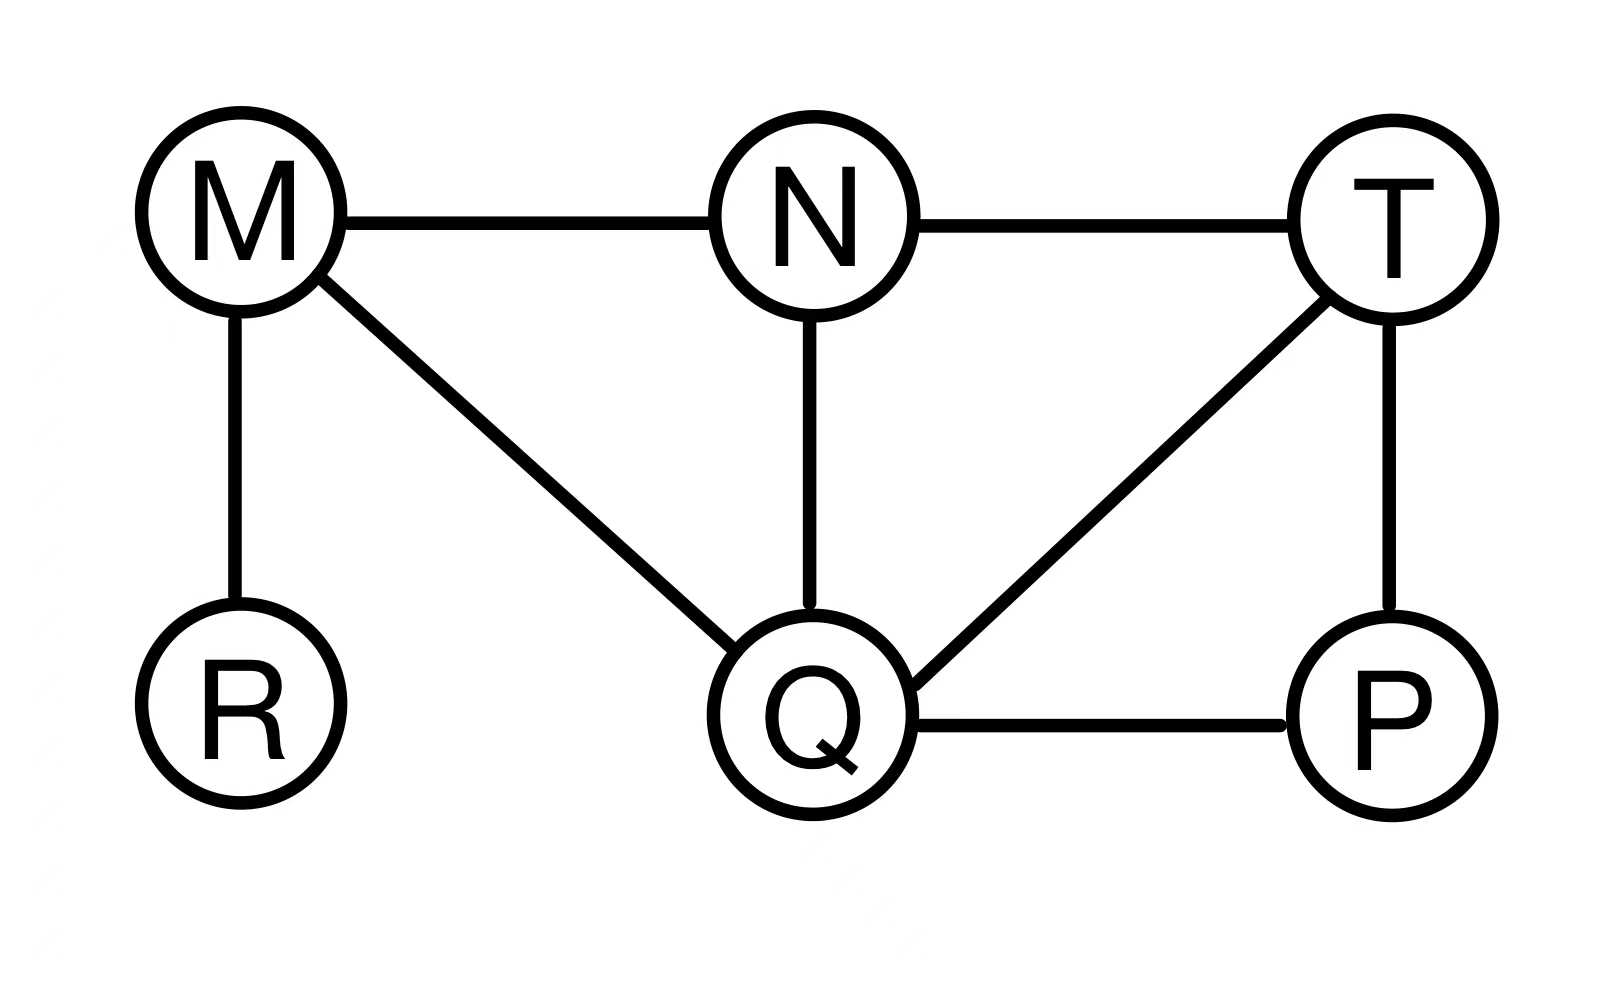
\includegraphics[width=.5\linewidth]{graph_search.png}
    \end{figure}
    \begin{enumerate}[A.]
        \item MNTPQR
        \item NQMPTR
        \item QMNRTP
        \item PTQNMR
    \end{enumerate}
    \begin{solution}
    D
    \end{solution}
    
    \item Let G be a directed graph whose vertex set is the set of numbers from 1 to 100. There is an edge from a vertex $i$ to a vertex $j$ if and only if either $j$ = $i$ + 1 or $j$ = 3$i$. The minimum number of edges in a path in G from vertex 1 to vertex 100 is
    \begin{enumerate}[A.]
        \item 23
        \item 99
        \item 4
        \item 7
    \end{enumerate}
    \begin{solution}
    D
    \end{solution}
\end{enumerate}

\section{Topological Sort (8 points)}
    In the lecture, we have introduced how to implement topological sorting algorithm by queue, whose main idea is quite similar to BFS. Mr. Blue Tiger argues that without \textbf{in−degree}, we can also implement topological sorting by using DFS, with an array \textbf{visited}. Complete the following pseudo code provided by him:
    \newline
    \newline
    \begin{algorithm}[htbp]
            \caption{Algorithm to implement topological sorting with DFS}
            \begin{algorithmic}[1]
                \STATE \textbf{Input:} an adjacency list representing the graph
                \STATE \textbf{Output:} a stack with the topologically sorted nodes.
                \STATE Create a stack $S$ and a boolean array $visited[]$ initialized with false.
                \FOR{each node $v$ in the graph}
                    \STATE dfs\_helper($v$, $visited$, $S$)
                \ENDFOR
                \newline
                \STATE dfs\_helper($v$, $visited$, $S$):
                \STATE // add codes here \textbf{if necessary}
                \newline
                \FOR{each node $u$ adjacent to $v$ }
                \IF{(! $visited[u]$)} 
                \STATE $S$.push($u$)
                \STATE $visited[u]\leftarrow true$
                \STATE dfs\_helper($u$,$visited$,$S$)
                \ENDIF
                \newline
                \ENDFOR
                \STATE // add codes here \textbf{if necessary}
            \end{algorithmic}
        \end{algorithm}

\section{Minimum Spanning Tree (12 points)}
\subsection{Delete an edge (6 points)}
Given a minimum spanning tree of a connected undirected graph G, an edge is deleted from G now. Suppose after deletion, G is still connected. Describe how to find the new minimum spanning tree with the old one in O(E) time.
\begin{solution}
If the original spanning tree does not contain the deleted edge, we do nothing. Otherwise,
for the vertex that is isolated, we search through all the edges that it connects
and pick the one with minimum weight.
\end{solution}

\subsection{Add an edge (6 points)}
Given a minimum spanning tree of a connected undirected graph G, an edge is added to G now. Describe how to find the new minimum spanning tree with the old one in O(V) time.
\begin{solution}
Say the added edge connects $u$ and $v$. Search through the unique path from 
$u$ to $v$ (one can use dfs to find such a path within $O(V)$ time since there are only $|V|-1$ edges),
find the edge with maximum weight. If it is larger than the weight of the newly added edge, then replace it.
\end{solution}

\section{Shortest Path (4 points)}
As introduced in the lecture, we can use Dijkstra's algorithm when the graph only has non-negative edges. Give a simple example of a directed graph with negative-weight edges for which Dijkstra's algorithm produces incorrect answers. Then briefly explain why Dijkstra's algorithm fails on your example.
\begin{solution}
\begin{figure}[H]
    \centering
    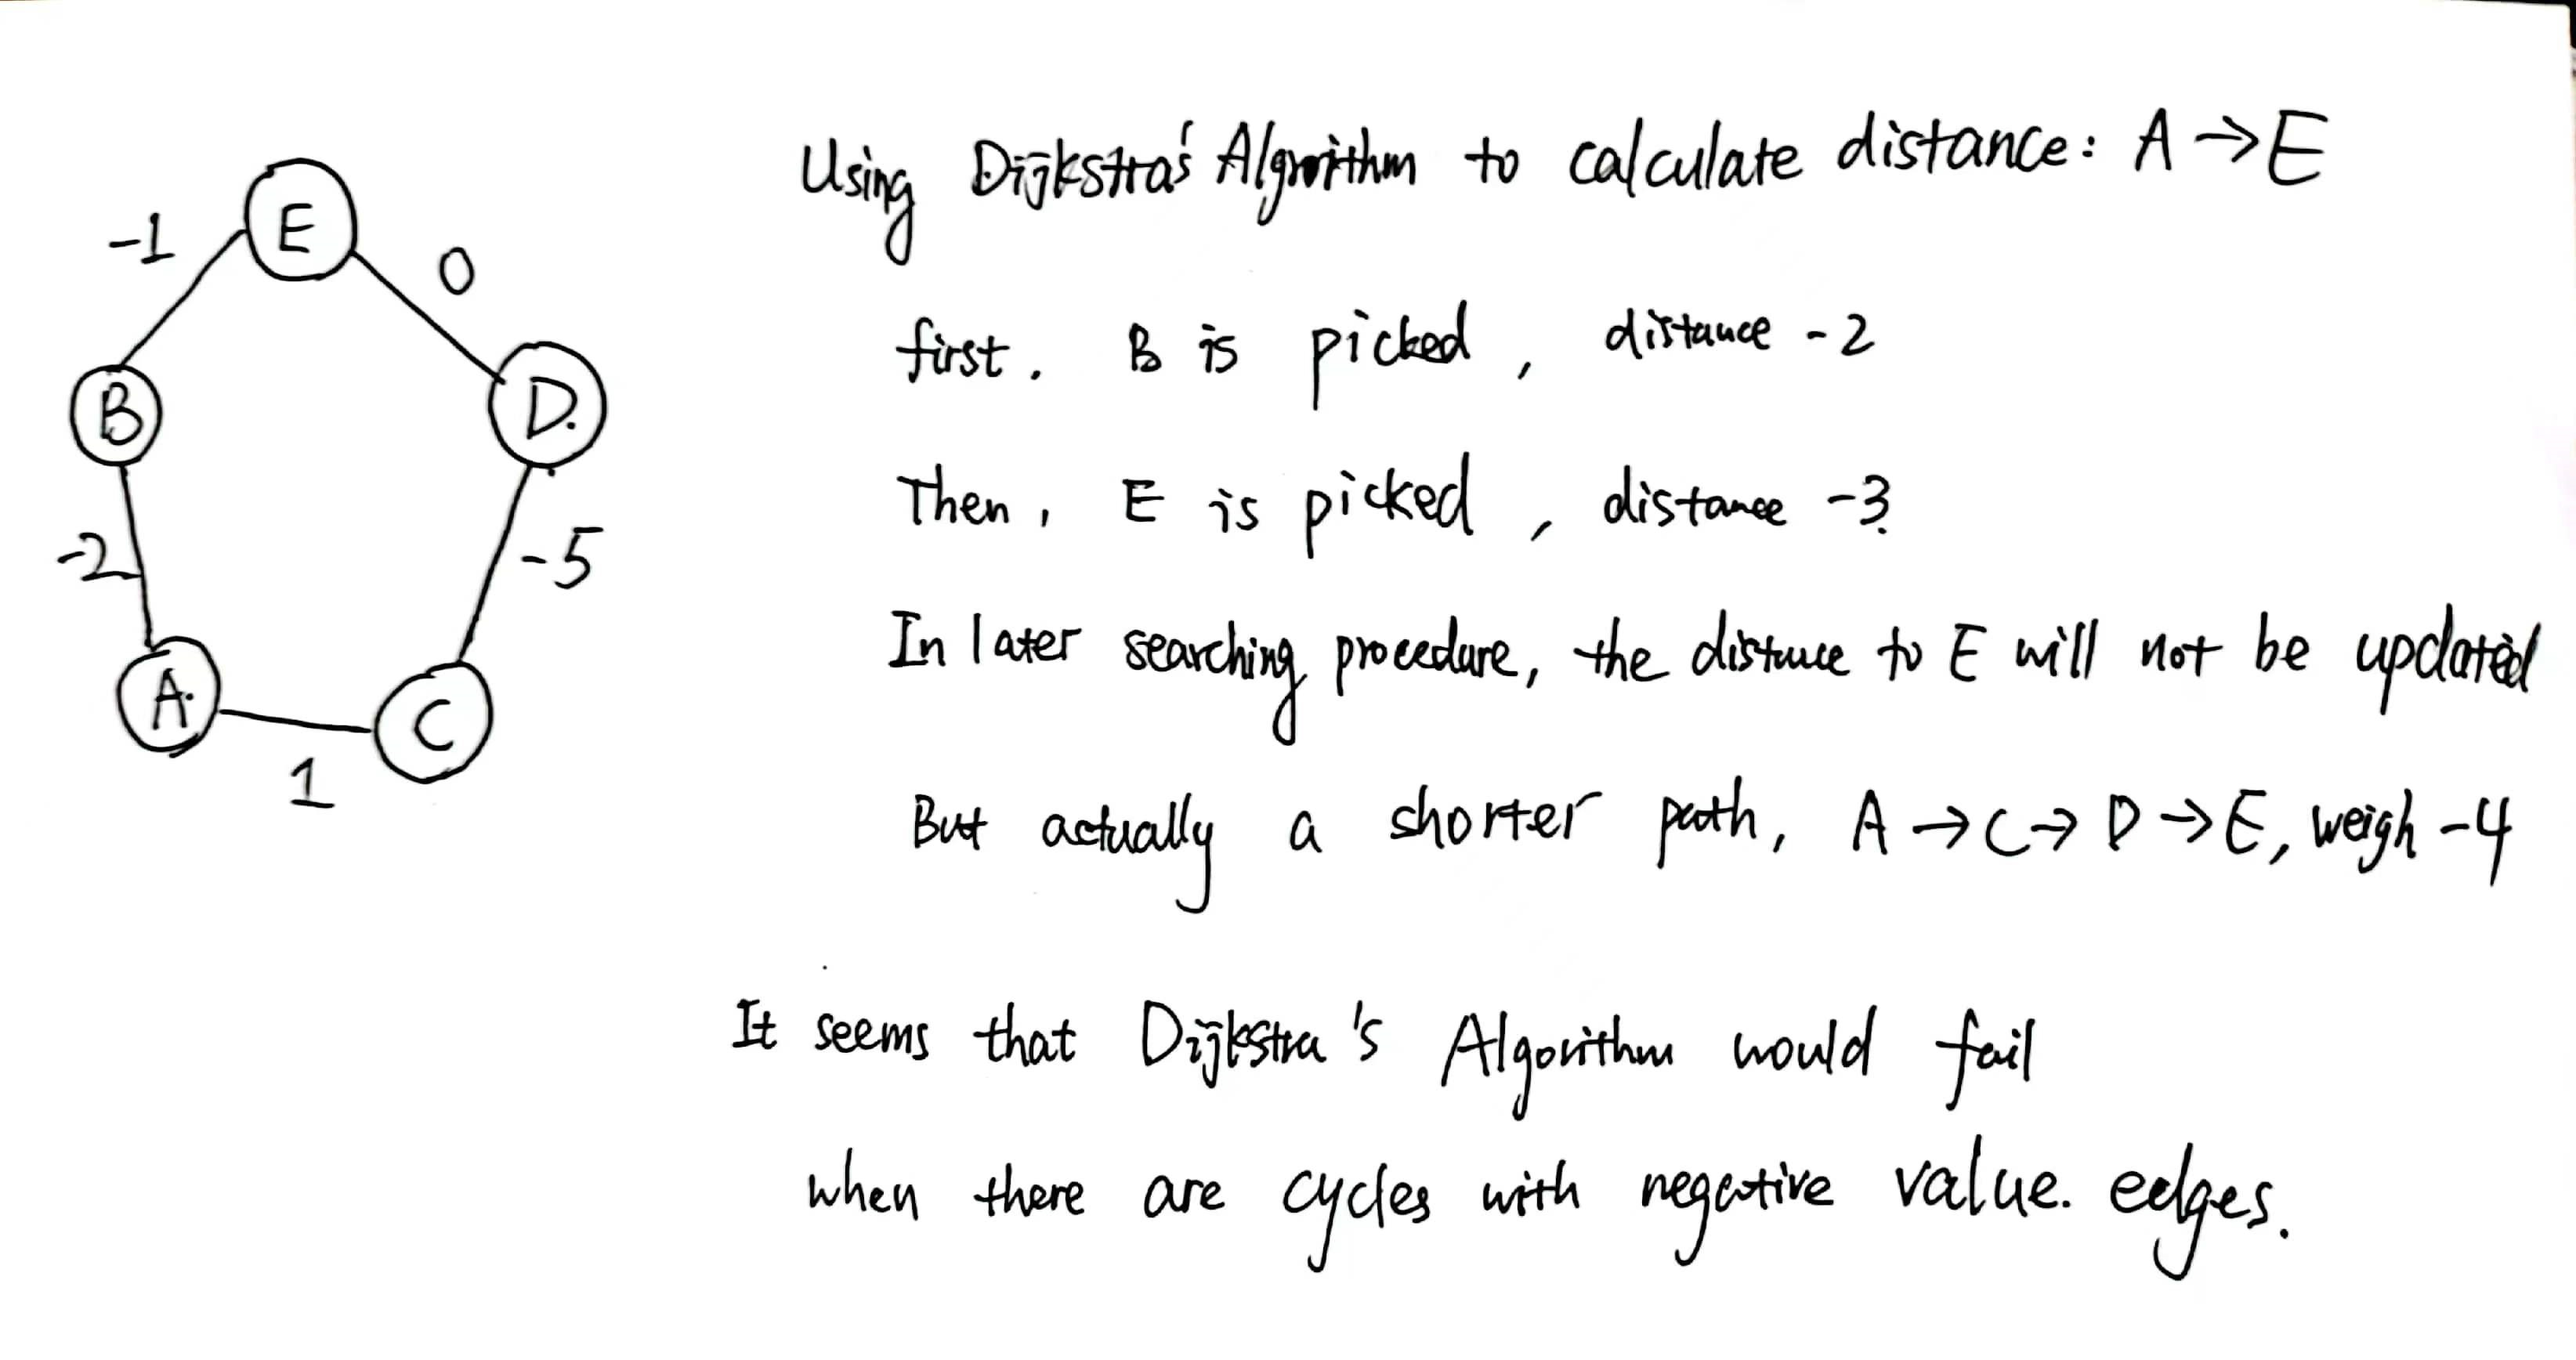
\includegraphics[width=0.95\linewidth]{hw4_4.jpg}
\end{figure}
\end{solution}

\section{Dynamic Programming (60 points)}
\subsection{Basic Case (12 points)}
\label{simple_repeat}
Suppose that we have an $n*n$ matrix filled with integers. Starting from the top left corner, we advance to either the downward or rightward block for each step and finally reach the bottom right corner of the matrix. During this process, we will pass through nodes with different integers. By applying dynamic programming, we can find the path with the largest sum of the passed integers. Write out the recurrence relation.
\begin{solution}
Suppose $a_{i,j}$ stands for the integer in $i$-th row, $j$-th column;
$f_{i,j}$ stands for the largest sum from the left corner to the block,
we have 
$$ f_{i,j} = \max \{f_{i-1,j}+f_{i,j-1}\} + a_{i,j}.$$
To find out the path, let $p_{i,j}$ stores the coordinate of previous block in the path
, then 
\begin{equation*}
    p_{i,j} = 
    \begin{cases}
        &p_{i-1,j}   \quad \quad ,f_{i-1,j}>f_{i,j-1}\\
        &p_{i,j-1}   \quad \quad ,f_{i-1,j}\leq f_{i,j-1}
    \end{cases}
\end{equation*}
\end{solution}
\subsection{Do it twice? (24 points)}
Previously, we just go across the matrix for a single time. Assume that after the first travel, we set the visited integer in the matrix to be 0 and go across the matrix, back to the left corner again. How to maximize the sum of the passed integers in the whole procedure (top left -> bottom right -> top left)? In terms of this problem, Alice and Bob have different ideas again.
\subsubsection{Simple repeat (10 points)}
Bob thinks that since this problem is quite similar to what we 
have solved in Section \ref{simple_repeat}, just run dynamic programming twice and add them up, and we will have the correct final result. Do you agree with him? If agree, write the recurrence relation for the second dynamic programming procedure and state whether there is a difference; if not agree, come up with a counter example and explain why it doesn't work.
\begin{solution}
No. Here is one counter example:\\
First round: 
\begin{equation*}
    \begin{pmatrix}
        \textcolor{red}{1} & 2 & 3\\
        \textcolor{red}{4} & \textcolor{red}{5} & 6\\
        7 & \textcolor{red}{8} & \textcolor{red}{9}
    \end{pmatrix}
\end{equation*}
Second round:
\begin{equation*}
    \begin{pmatrix}
        0 & \textcolor{blue}{2} & \textcolor{blue}{3}\\
        0 & 0 & \textcolor{blue}{6}\\
        7 & 0 & 0
    \end{pmatrix}
\end{equation*}
However, the largest path would be ({\color{red} top left -> bottom right}, {\color{blue} bottom right -> top left}):
\begin{equation*}
    \begin{pmatrix}
        \textcolor{red}{1} & {2} & {3}\\
        \textcolor{red}{4} & 5 & {6}\\
        \textcolor{red}{7} & \textcolor{red}{8} & \textcolor{red}{9}
    \end{pmatrix}
    + 
    \begin{pmatrix}
        0 & \textcolor{blue}{2} & 3\\
        0 & \textcolor{blue}{5} & \textcolor{blue}{6} \\
        0 & 0 & 0
    \end{pmatrix}
\end{equation*}
\end{solution}
\subsubsection{Double the result table (14 points)}
Alice thinks that the dynamic programming strategy for this problem should be modified from the very beginning in this case. She gives out the main function as shown below. However, after testing, she found out there are some problems within this piece of code. Please correct the code between line 17 to line 26.
\newpage 
\begin{lstlisting}
int main(){
    // two paths are considered simultaneously, one at (i, j), the other at (k, l)
    // integers stored in integer[n][n]
    int n;
    cin >> n;
    int dp[100][100][100][100] = {0};
    int integers[100][100] = {0};
    // read all the inputs
    for (int i = 1; i <= n; i++)
        for (int j = 1; j <= n; j++)
            cin >> integers[i][j];
    
    dp[1][1][1][1] = integers[1][1]; // start point
    
    // start dp
    
    /* modify code within this part */

    for (int i = 1; i <= n; i++)
        for (int j = 1; j <= n; j++)
            for (int k = 1; k <= n; k++)
                for (int l = 1; l <= n; l++){
                    dp[i][j][k][l] = max(dp[i-1][j][k-1][l], dp[i][j-1][k-1][l],
                                         dp[i-1][j][k][l-1], dp[i][j-1][k][l-1])
                                         + integers[i][j] + integers[k][l];
                    if(i==k&&j==l) dp[i][j][k][l]-=integers[i][j];
                }                         
                                         
    /* modify code within this part */
    
    cout << dp[n][n][n][n];
    
}
\end{lstlisting}
\subsection{How to save memory? (12 points)}
Bob takes a look at Alice's strategy and thinks that its memory usage is too bad. Regardless of correctness, it will have a space complexity of $O(n^4)$, which sounds horrible. Propose a modification to this dynamic programming algorithm so that the space complexity can be reduced to $O(n^3)$ and write out its recurrence relation.\\
Hint: one way to do so is to reduce the array $dp$ to be 3-dimensional. There should be 1 dimension still for $i$ and 1 dimension still for $k$.
\begin{solution}
Let $dp[l][i][k]$ represents the total sum that the length of current path is $l$, with the 
first path reaches $(i,l-i)$, the second path reaches $(k,l-k)$.\\
Now, we enumerate $l$ from $1$ to $2n$, $i$ from $1$ to $n$, $k$ from $1$ to $n$, with the dp equation
\ttfamily{
    dp[l][i][k] = max(dp[l-1][i-1][k-1], dp[l-1][i][k-1],
    dp[l-1][i-1][k], dp[l-1][i][k])
    + integers[i][l-i] + integers[k][l-k];
}
Of course the situation that \ttfamily{(i==k)} needs to be considered like above.
\end{solution}
\subsection{Does optimization end here? (12 points)}
Looking at the modification proposed by Bob, Alice surprisingly agrees with him. After brainstorming, they find that this strategy can be further optimized in terms of space complexity. Briefly state how you can further reduce its space complexity to $O(2n^2)$.\\
Hint: Do we need every $dp$ value in every iteration?
\begin{solution}
Since in every iteration we only need the value of $dp[l-1][][]$, we can reduce the array to be $2\times n\times n$.
Namely $dp[1][i][k]$ represents all the states that the length are odd and $dp[2][i][k]$ represents
all the states that the length are even. Now the dp equation can be rewritten into:\\
\ttfamily{
    dp[l\%2][i][k] = max(dp[(l-1)\%2][i-1][k-1], dp[(l-1)\%2][i][k-1],
    dp[(l-1)\%2][i-1][k], dp[(l-1)\%2][i][k])
    + integers[i][l-i] + integers[k][l-k];
}
\end{solution}
Notes: Actually we can further reduce its space usage from $O(2n^2)$ to $O(n^2)$ in this problem.
\newpage

\section*{Reference}
Assignment 4, VE281, FA2021, UMJI-SJTU

Assignment 5, VE281, FA2021, UMJI-SJTU

Algorithms, 4th Edition by Robert Sedgewick and Kevin Wayne, Princeton University
\end{document}